\begin{center}
    {\LARGE \textbf{2005物理化学}} \\[2ex]
    {\large 时量180分钟 \quad 满分90分}
\end{center}

\vspace{0.5cm}
\noindent\textbf{注意事项:}
\begin{enumerate}[label=\arabic*., parsep=0pt, itemsep=0pt]
    \item 答题前,考生先将自己的姓名、学号、考场号、座位号填写在答题卡上,将条形码准确粘贴在考生信息条形码粘贴区。
    \item 考试结束后,将本试卷与答题纸一并收回。
    \item 回答各个问题时,将答案写在答题纸上,写在本试卷上无效。
\end{enumerate}

\vspace{0.5cm}
\noindent\textbf{1. (15 pts.)}

$5\ \mathrm{mol}$单原子分子理想气体始态的温度为$373.6\ \mathrm{K}$，压力为$2.750\ \mathrm{MPa}$，经绝热不可逆过程到达终态。该过程的$\Delta S_m = 20.92\ \mathrm{J\cdot K^{-1}\cdot mol^{-1}}$，$W = -6.275\ \mathrm{kJ}$。已知$S_m(373.6\ \mathrm{K}) = 167.4\ \mathrm{J\cdot K^{-1}\cdot mol^{-1}}$，求终态的$p_2,V_2,T_2$及过程的$\Delta U,\Delta H,\Delta G,\Delta F$。

\vspace{0.5cm}
\noindent\textbf{2. (15 pts.)}

在$660.7\ \mathrm{K}$时，金属$\ce{K}$和$\ce{Hg}$的蒸气压分别是$433.2\ \mathrm{kPa}$和$170.6\ \mathrm{kPa}$，在$\ce{K}$和$\ce{Hg}$的物质的量相同的溶液上方，$\ce{K}$和$\ce{Hg}$的蒸气压分别为$142.6\ \mathrm{kPa}$和$1.733\ \mathrm{kPa}$，设以纯液体$\ce{K}$和$\ce{Hg}$为标准态，计算
\begin{enumerate}[label=(\arabic*), itemsep=1ex]
    \item $\ce{K}$和$\ce{Hg}$在溶液中的活度和活度因子；
    \item 若$\ce{K}$和$\ce{Hg}$分别为$0.5\ \mathrm{mol}$，计算它们的$\Delta_\mathrm{mix}G,\Delta_\mathrm{mix}S$和$\Delta_\mathrm{mix}H$。
\end{enumerate}

\vspace{0.5cm}
\noindent\textbf{3. (15 pts.)}

将$1.1\ \mathrm{g}\ \ce{NOBr}$放入$-55^\circ\mathrm{C}$抽成真空的体积为$1\ \mathrm{L}$的容器中加热到$25^\circ\mathrm{C}$，此时容器内均为气态物质，总压力为$32424\ \mathrm{Pa}$，其中存在以下化学平衡：
\[
\ce{2NOBr <=> 2NO + Br_2}
\]
将容器内的气体视为理想气体，求上述反应在$25^\circ\mathrm{C}$时的标准自由能$\Delta_\mathrm{r}G_\mathrm{m}^\ominus$。
已知摩尔质量：$\ce{N}$:$14\ \mathrm{g\cdot mol^{-1}}$，$\ce{O}$:$16\ \mathrm{g\cdot mol^{-1}}$，$\ce{Br}$:$80\ \mathrm{g\cdot mol^{-1}}$。

\vspace{0.5cm}
\noindent\textbf{4. (15 pts.)}

某一级反应在$450\ \mathrm{K}$和$500\ \mathrm{K}$时速率常数分别为$3.67\times10^{-7}\ \mathrm{s^{-1}}$和$5.12\times10^{-5}\ \mathrm{s^{-1}}$，求该反应的活化能$E_\mathrm{a}$和$500\ \mathrm{K}$时的活化熵$\Delta^\neq S_\mathrm{m}^\ominus$、活化焓$\Delta^\neq H_\mathrm{m}^\ominus$。

\vspace{0.5cm}
\noindent\textbf{5. (15 pts.)}

电池$\ce{Pt,H_{2}}(g)(p^\ominus)|ce{NaOH}(溶液)|ce{HgO}(s),ce{Hg}(l),ce{Pt}$在$298\ \mathrm{K}$时的电动势$E = 0.9261\ \mathrm{V}$。
已知$\Delta_\mathrm{f}H_\mathrm{m}^\ominus(\ce{HgO,s}) = -90.71\ \mathrm{kJ\cdot mol^{-1}}$，$\Delta_\mathrm{f}H_\mathrm{m}^\ominus(\ce{H_{2}O,l}) = -285.84\ \mathrm{kJ\cdot mol^{-1}}$。
\begin{enumerate}[label=(\arabic*), itemsep=1ex]
    \item 写出电极反应与电池反应，设反应电子数为$2$；
    \item 求$298\ \mathrm{K}$时电池反应的平衡常数；
    \item 求$308\ \mathrm{K}$时电池的电动势$E$。
\end{enumerate}

\vspace{0.5cm}
\noindent\textbf{6. (15 pts.)}

\begin{enumerate}[label=(\arabic*), itemsep=1ex]
    \item 求$\ce{NO(g)}$在$298.15\ \mathrm{K}$及$101325\ \mathrm{Pa}$时的摩尔熵。已知$\ce{NO}$的$\Theta_r = 2.42\ \mathrm{K},\Theta_v = 2690\ \mathrm{K}$，电子基态和第一激发态简并度皆为$2$，二能级间隔$\Delta\varepsilon = 2.473\times10^{-21}\ \mathrm{J}$。
    \item 下图是二组分体系的固液平衡相图。根据相图回答下列问题：
    
    \begin{figure}[htbp]
        \centering
        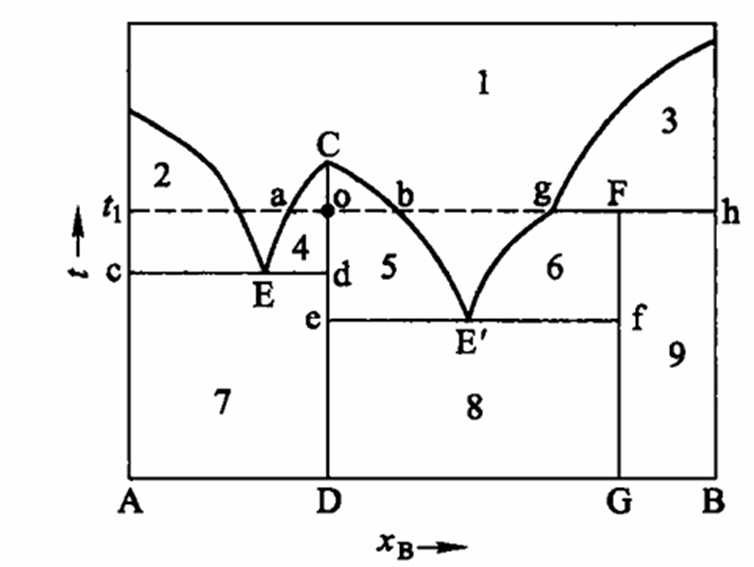
\includegraphics[width=0.6\textwidth]{./Figure/P_2005_6}

    \end{figure}

    \begin{enumerate}[label=(\alph*), itemsep=1ex]
        \item 列表写出用数字标识的各相区的相的组合；
        \item 列表写出$\mathit{cd},\mathit{ef},\mathit{gh},\mathit{CD},\mathit{FG}$各线所代表的体系的相数、相态与自由度；
        \item 在温度为$t_1$时，$\mathit{a}$点可以与$\mathit{o}$点平衡共存，$\mathit{b}$点也可以与$\mathit{o}$点平衡共存。$\mathit{a}$点与$\mathit{b}$点二者可否平衡共存？为什么？
    \end{enumerate}
\end{enumerate}